\eat{
\subsection{}
\footnote{}
\emph{}
\texttt{} 
~\cite{}
~\ref{sec:}

}


\section{Motivation and Challenge}
\label{sec:moch}

% There is a growing trend toward systems in multiple distributed locations that
% generate massive amounts of data. From sensor networks to traffic monitoring
% systems, and from email spam generators to network firewalls --- these distributed systems
% "fabricate" data at volumes that prohibit
% centralized processing. Furthermore, these environments often require
% decentralized active control or decision making because they cannot rely on a
% centralized master. We are challenged to assemble the uncertain and
% distributed raw data into "information-products". In other words, we must
% perform probabilistic inference with the representation and computation
% distributed across many nodes. For instance, we want to perform classification
% on network firewall data patterns to predict an attack. We are thusly
% motivated to design software infrastructures that support the easy
% implementation of algorithms for inference in networked systems, as well as
% new algorithms for reasoning over large-scale distributed information sources.
% 
% In this report, we demonstrate how probabilistic inference algorithms can be
% implemented concisely in a distributed manner. Using P2, a framework for
% declarative networking and OverLog, its language (a Prolog-variant for
% distributed queries), we prototype such a declarative inference system with a
% distributed Junction Tree algorithm based on the work by Paskin et al \cite{ipsn}.
% 
% The benefits of our approach are several. Our declarative approach yielded
% more than 10x reduction in lines of code compared to the Lisp implementation
% by Paskin et al \cite{ipsn}. The OverLog language allows high-level
% logical specification of algorithms with embedded network semantics, which is
% modular and pedagogically interesting. Our algorithm is simplified from that
% of Paskin et al. We implemented some similar robustness features, such as
% having the communication layers automatically update on failure and
% recovery. These characteristics, together, recommend our approach and suggest
% that variations of inference algorithms can be easily implemented, deployed,
% tested and compared on this framework. 

There is a growing trend toward systems in multiple distributed locations that
generate massive amounts of data. These systems can often take advantage of
learning and inference algorithms to improve their operation. For example,
internet routers may perform classification on network firewall data patterns
to predict an attack. Unfortunately, the high amount of of data generated at
the network locations often prohibits centralized processing. This challenge
motivates the design of decentralized inference algorithms that distribute the
representation and computations across several nodes in the network. Such
algorithms are also useful when in active control applications when nodes wish
to make decisions based on partial results computed at any point in time.

Simple algorithms, such as loopy belief propagation distribute naturally
\cite{loopy}. In these algorithms, there is typically a one-to-one mapping
between the nodes and the variables in the network, and nodes can perform the
computations in an entirely local manner. However, more complex algorithms,
such as the robust distributed inference algorithm by Paskin et al.
\cite{ipsn} require additional coordination that makes programming using
message-passing style algorithms tiresome and error-prone.

In this project, we demonstrate that declarative approaches, in particular, P2
\cite{p2}, can substantially simplify the design and implementation of
distributed inference algorithms. P2 is a framework for declarative network
programming that uses a variant of Prolog to describe the algorithm and its
behavior. We wrote a prototype P2 implementation of the inference architecture
in \cite{ipsn} that was then used to compute marginal probability queries on a
Gaussian Markov random field (MRF). Our implementation contains the key
features of the architecture, including robustness to node loss and
re-adaptation of the network junction tree in presence of changing link
conditions. Our implementation is substantially shorter (by a factor of ten)
than the reference Lisp implementation by Paskin et al. We tested our
implementation on the RAD Lab cluster, demonstrating scalability and ease of
deployment.


% \section{Approach and Solution}
% \label{sec:apso}
% 
% \paragraph{P2 and benefits} We use P2, a declarative networking system as the
% basis for our distributed programming and runtime infrastructure. We include a
% brief review here. For more details see \cite{p2}. P2 executes distributed
% algorithms specified in a high level language, OverLog. The language is based
% on Datalog, a logic programming language. OverLog programs are constructed
% from rules which specify how facts are generated from each other. Key concepts
% are relations and fact tuples. A relation is described by a list of fields,
% and a fact tuple is an assignment of values to the fields. There are two types
% of relations, materialized and streaming. Materialized relations are like
% database tables and streaming relations are like events. OverLog programs are
% well suited for specifying distributed inference algorithms, which basically
% involve maintaining lists of neighbors and passing messages between the
% neighbors. In the P2 runtime, the OverLog rules are compiled into a dataflow
% graph, which is instantiated on each node. A dataflow is an optimized
% specification of the resulting distributed application, which handles message
% passing, relational operations such as \emph{(join, selection, projection,
% aggregation)}, queueing, multiplexing, etc. Using this system, we prototype an
% existing set of algorithms and extend P2 where necessary to
% more-naturally support inference.

\section{Declarative approach to distributed inference}
\label{sec:apso}

\paragraph{P2 and its benefits} We use P2, a declarative networking system as
the basis for our distributed programming and runtime infrastructure. We
briefly review P2 here; for more details, see \cite{p2}.

P2 executes distributed algorithms specified in logical programming language,
OverLog, which is based on Datalog. OverLog programs are constructed from
rules which specify how facts are generated from each other. Key concepts are
relations and fact tuples. A relation is described by a list of fields, and a
fact tuple is an assignment of values to the fields. There are two types of
relations, materialized and streaming. Materialized relations are like
database tables and streaming relations are like events. OverLog programs are
well suited for specifying distributed inference algorithms -- these
algorithms often often maintain local information relative to each node, such
as list of its neighbors and incoming messages, and this information can be
effectively maintained and manipulated in a relational table.

In the P2 runtime, the OverLog rules are compiled into a dataflow graph, which
is instantiated on each node. A dataflow is an optimized specification of the
resulting distributed application, which handles message passing, relational
operations such as \emph{(join, selection, projection, aggregation)},
queueing, multiplexing, etc. Using this system, we wish to prototype existing
algorithms and extend P2 as needed.

\begin{figure}[htpb]
 \centering
 \epsfxsize=1in
 \includegraphics[width=3in]{figs/architecture-summary.eps}
 \caption{Layered graphs for distributed inference. The top two layers are implemented by a distributed inference algorithm; the lower layer is the physical network.}
 \label{fig:architecture}
\end{figure}

\paragraph{Architecture} Our implementation of distributed Junction Tree
algorithm is based on the architecture of Paskin et al \cite{ipsn}. The
architecture involves implementing three layers:

\begin{enumerate}

\item {\textit{Spanning tree layer:}} This layer allows each node in the
network to connect with a set of nodes such that all the nodes in the network
form a spanning tree. The cost function to choose a link can be changed as per
the scenario.

\item{\textit{Junction tree layer:}} Once the nodes are connected in the form
of a spanning tree, they can communicate with their neighbors to transfer
information about the variables they carry or their neighbors carry. Using
this information nodes are able to compute the variables they can reach and
thus achieve the running intersection property (refer to listing 1 for rules).
Nodes determine their clique in this layer.

\item{\textit{Inference layer:}} The inference layer would allow the nodes to
transfer messages between themselves to calculate the probabilistic inference
at a particular node. For example, in the case of probabilistic inference,
each node starts with a potential over (a subset of) its clique $C_i$. Each
node $i$ then computes the inference message $\mu_{ij}$ to its neighbor node
$j$ based on the messages received from its other neighbors $k$.

\[
\mu_{ij} = \sum_{C_i \setminus S_{ij}} \psi_{C_i} \prod_{k \neq i} \mu_{ki}
\]

Once the node $i$ has received messages from all of its neighbors, we compute
the marginal probability update for i:

\[
p(C_i) \propto \psi_{C_i} \prod_{k} \mu_{ki}
\]

\end{enumerate}	

Compared to a traditional centralized approach where the core of the algorithm
is a triangulated graph based on running variable elimination, our three
layers run at the same time, and should respond to changes between the layers.
This is because in a distributed environment, one cannot assume that the
physical nodes are stable and know when the communication graph has
stabilized. For instance, when a node fails, the spanning tree detects the
event, removes the node, and the junction tree updates its cliques. Similarly,
for a new node joining the inference network, the trees are updated
accordingly. The dynamic updates help in calculating accurate probabilistic
inference as per the latest network. However, this means the communication and
computational complexity is not globally minimized. As the Paskin et al. work
suggests, a locally optimized junction tree gives meaningful and performant
results.

\paragraph{Algorithms}

To give you a feel of declarative rules and their conciseness we briefly
explain the rules of junction tree and spanning tree algorithms. Refer to the
Appendix for more details.

\emph{The Junction tree Overlog} contains five rules to satisfy running
intersection property across remote nodes in a distributed network. Each node
has a \textit{clique} relation that stores the clique information of that
node. The \textit{reachable} relation stores information of the variables a
node can reach from its neighbor \textit{Nbr}.

\emph{The Spanning tree OverLog} contains six rules which compute minimum cost
communication paths. Each node stores the best paths to all neighbors, and
propagates the information periodically. When a node receives an update with
better path, it changes its path accordingly.

\section{Experiment and Results}
\label{sec:exre}

To evaluate our algorithms and architecture we used the same data set as
Paskin et al. 54 sensors were deployed at the Intel-Berkeley lab, and
collected temperature readings over a period of time. A Markov Random Field
model was fit to this data where each node has a unobserved temperature random
variable. The joint probability model is given by

\[
p(T_1, T_2, ..., T_n) \propto \prod_{i,j \in E} \psi_{ij}(T_i, T_j)
\]

We assign potentials of the Markov Random Field to the cliques at each node.
For the assignment we take a greedy approach and assign pair-wise potential to
nodes such that there is a balance of variables at each node across the
network.

We reproduced the experiment on the RAD lab cluster, running on networks of 4,
10 and 54 nodes.

\paragraph{Spanning tree experiment} To validate the robustness and adaptivity
of our spanning tree algorithm we ran the spanning tree algorithm on a 10 node
network, see Figure~\ref{fig:spanntree_robustness}. At the beginning of the
experiment we waited until the spanning tree became stable. After
stabilization, we simulated node failure and network bisection, and found that
the spanning tree updated to reform two spanning trees. Once the spanning tree
stabilized again, we brought the nodes that were dead back alive to simulate
recovery from node failures. Our evaluation found that the spanning tree
updated to include the newly alive nodes.

\begin{figure}[hptb]
 \centering
 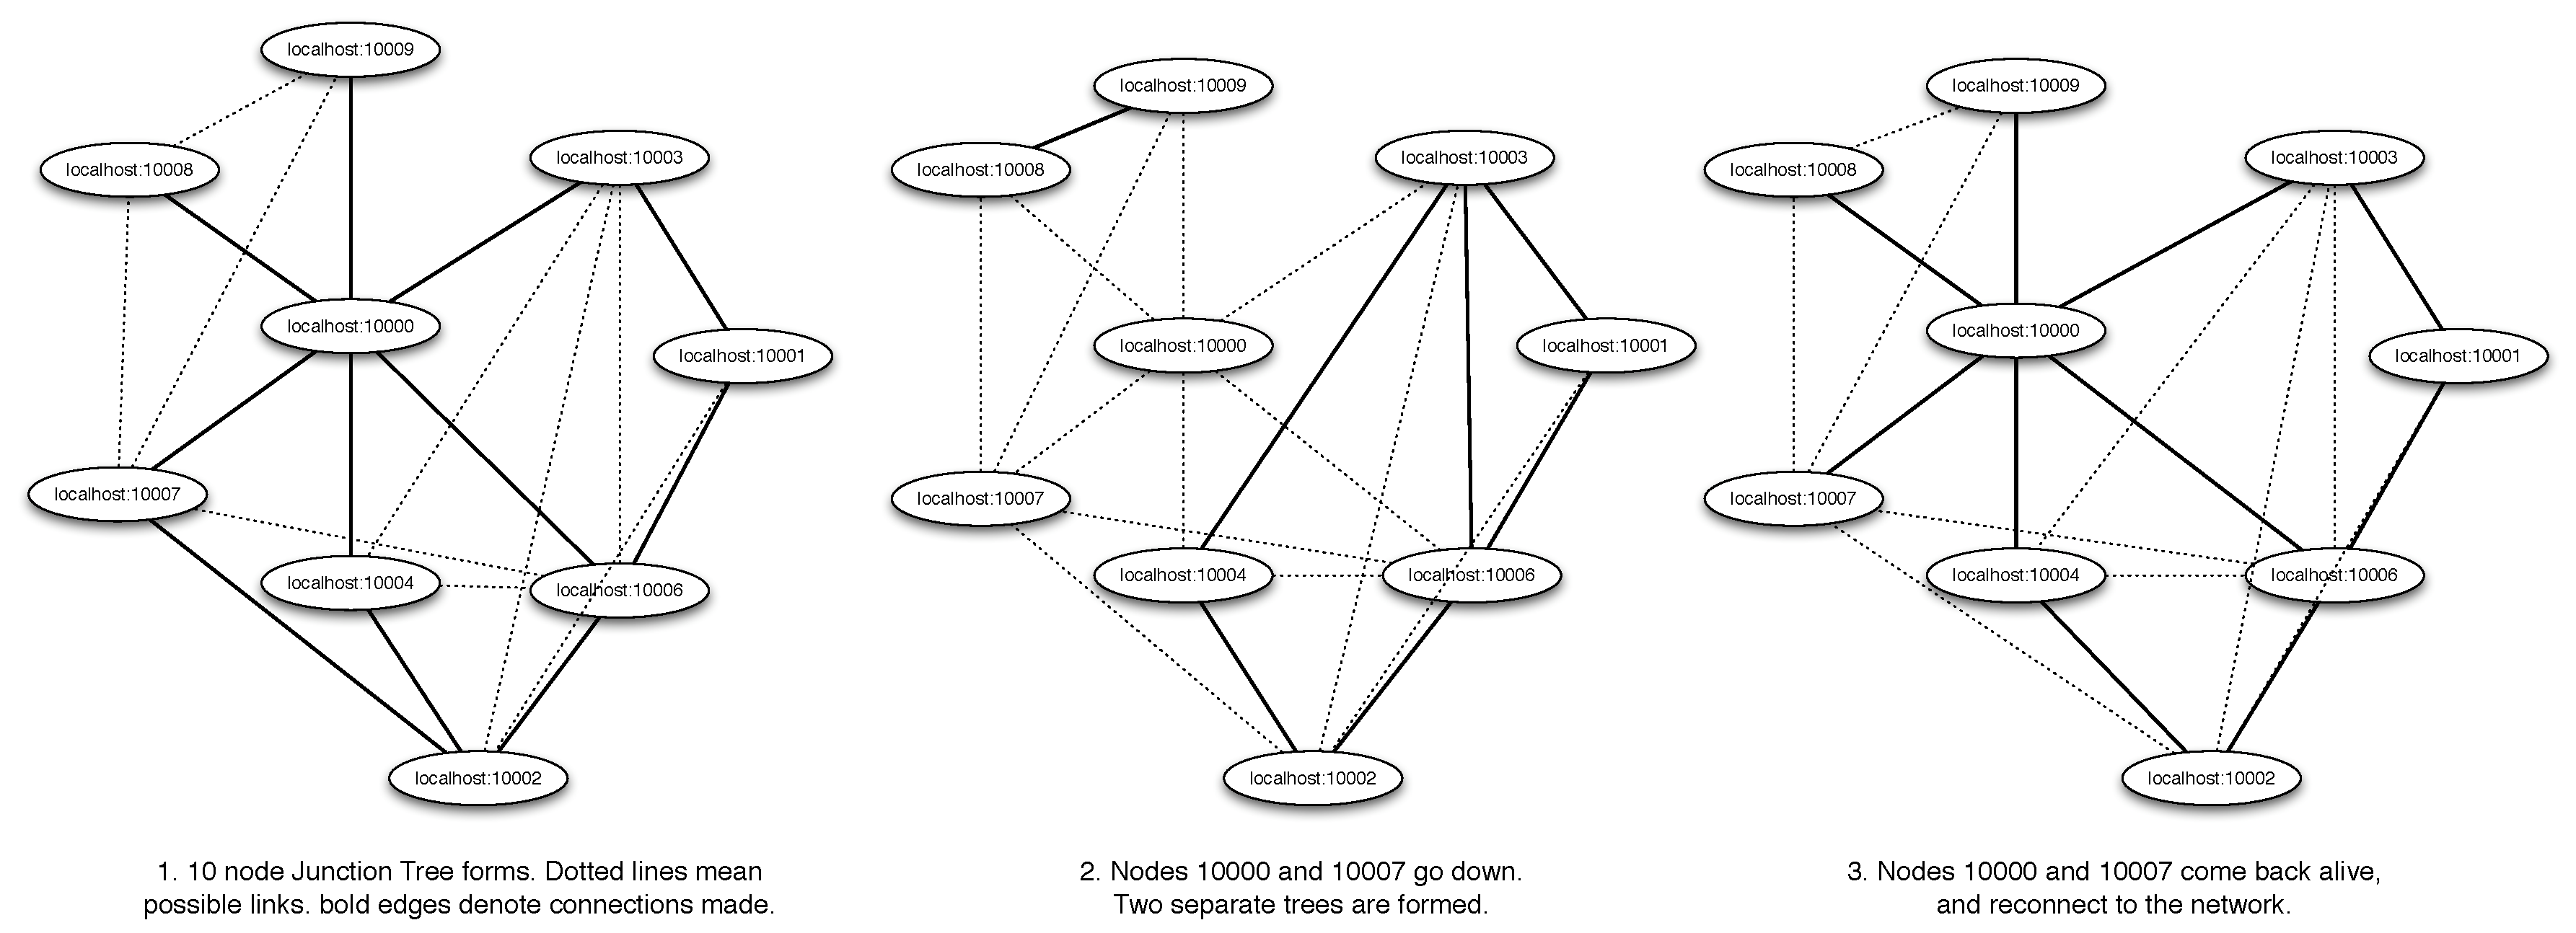
\includegraphics[width=\columnwidth]{figs/spantree_robustness.eps}
 \caption{Graph state progression during node failure and recovery.}
 \label{fig:spanntree_robustness}
\end{figure}

\paragraph{Junction tree experiment} In order to evaluate the performance of
junction tree algorithm we measured the time it took for each node to
stabilize their clique membership in a 54 node network.
Figure~\ref{fig:performance} shows that the maximum time taken by a node in
the network was less than 16 seconds. The nodes that took the longest time
were nodes that have a large clique. On average a node took around two seconds
to arrive at a stable clique. The nodes with zero clique stabilization time
were nodes whose cliques were same as their initial clique.

\begin{figure}[htpb]
 \centering
 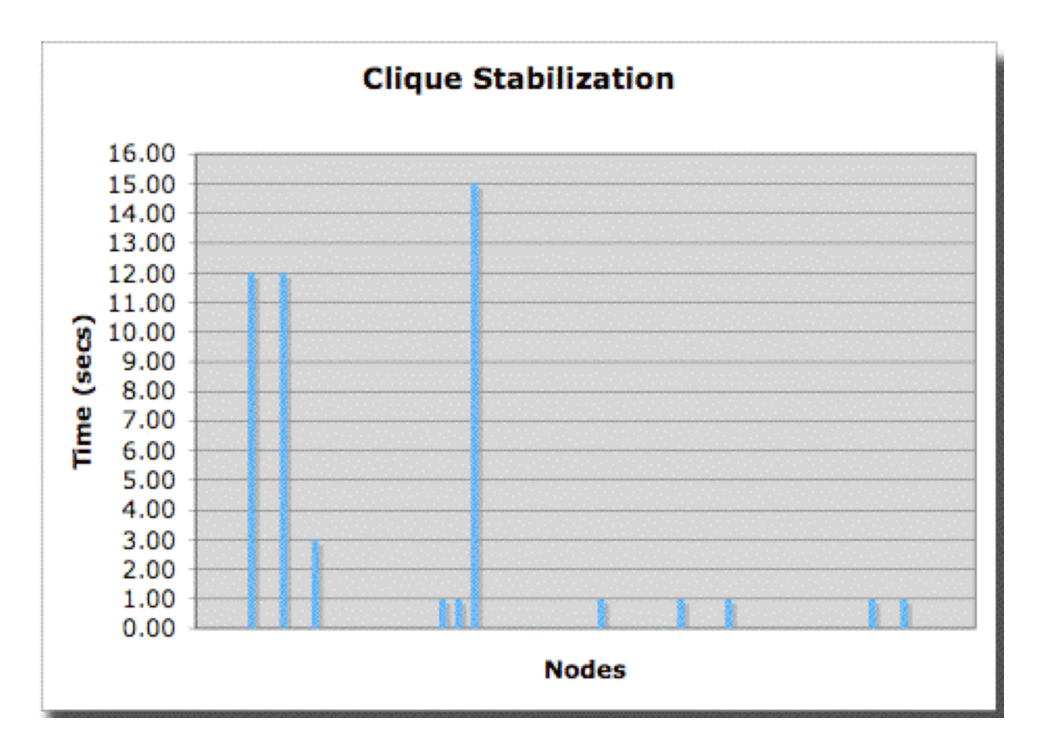
\includegraphics[width=3in]{figs/performance.eps}
 \caption{Junction tree clique calculation and stabilization times per node.}
 \label{fig:performance}
\end{figure}

We also verified whether the running intersection property holds true in case
of the 54 node network with a program which polled the distributed nodes and
independently calculated the resulting cliques. Refer to the Appendix for the
resulting network graph and cliques.

\paragraph{Inference algorithm} The distributed experimental runs calculated
the nodes' marginal probabilities over each node's temperature. We verified
the Gaussian means of the node temperature with a Matlab program for the same
dataset.

\section{Conclusion}
\label{sec:conc}

In this project, we have taken a first step towards establishing the fitness
of a declarative approach to distributed inference. Our approach allows for
easy prototyping, evaluation, and design iteration of other inference
algorithms. We first identified existing algorithms and implemented them ---
showing the compactness and efficiency of our approach. Next, we evaluated
various robustness measures. We found a race condition in the original
algorithm (whereby nodes could propagate stale information indefinitely) and
was able to address it easily --- illustrating both a crucial feature of
distributed inference algorithms, and an effective expressiveness in our
declarative language. Then, we evaluated the system on a 54 node data set of a
comparable implementation with the RAD Lab cluster --- verifying the
correctness of inference results and performance for forming the networked
data structures for inference.

In future work, we plan to implement other inference algorithms, such as loopy
belief propagation \cite{loopy} and other approximate algorithms, and compare their
complexity of implementation, performance and robustness. 

Other interesting next steps are to try out other machine learning algorithms,
such as regression and classification. As well, it would be useful to
investigate algorithms for mapping graphical models to network nodes.
